\subsubsection{Non-autonomous scalar problem}
\label{sec:appendix_verification_nonautonomous}
\begin{figure}[!b]
    \centering
    \begin{minipage}[t]{0.48\textwidth}
        \centering
        \vspace{0pt}
        % This file was created by matlab2tikz.
%
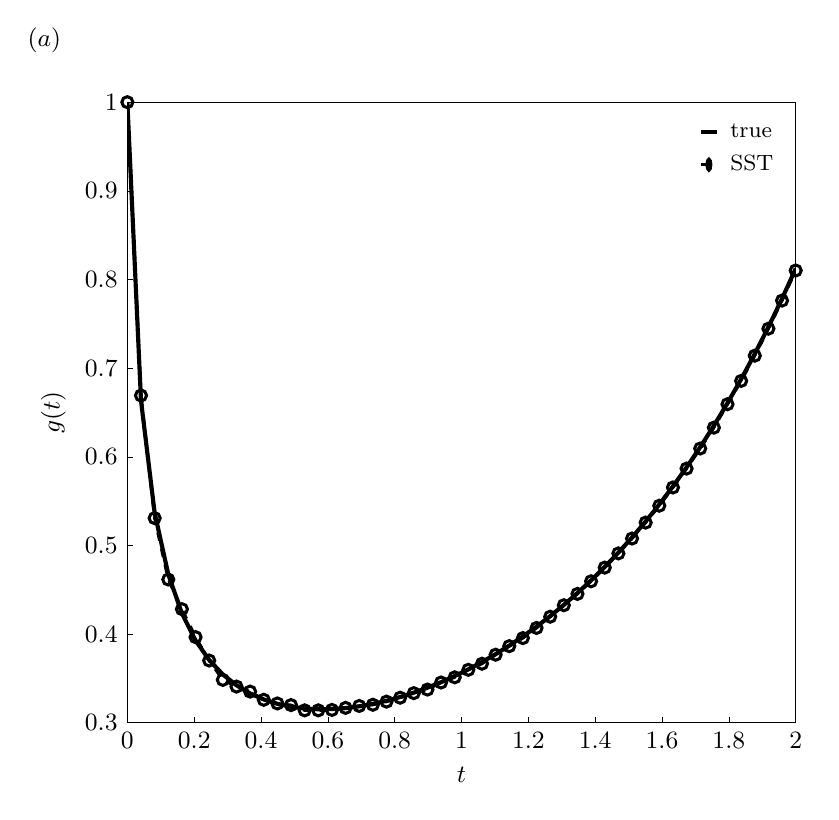
\begin{tikzpicture}

\begin{axis}[%
width=11.252in,
height=7.131in,
at={(1.887in,0.962in)},
scale only axis,
clip=true,
separate axis lines,
every outer x axis line/.append style={black},
every x tick label/.append style={font=\color{black}},
every x tick/.append style={black},
xmin=0,
xmax=2,
xlabel={$t$},
every outer y axis line/.append style={black},
every y tick label/.append style={font=\color{black}},
every y tick/.append style={black},
ymin=0.3,
ymax=1,
ylabel={$g(t)$},
axis background/.style={fill=white},
legend style={legend cell align=left, align=left},
clip=true,
clip mode=individual,
axis lines=box,
xtick pos=bottom,
ytick pos=left,
tick align=inside,
major tick length=2pt,
width=0.7\linewidth,
height=0.65\linewidth,
every axis/.append style={font=\fontsize{9}{9}\selectfont},xlabel style={font=\fontsize{9}{9}\selectfont},title style={font=\fontsize{9}{9}\selectfont},
legend style={font=\fontsize{8}{9}\selectfont,inner sep=1pt,row sep=1pt,column sep=2pt,nodes={scale=1.00},draw=none},legend image post style={xscale=0.35},
legend columns=1,
scaled x ticks=false,
tick label style={/pgf/number format/fixed,/pgf/number format/precision=2},
every x tick label/.append style={font=\fontsize{9}{9}\selectfont\color{black}},
every y tick label/.append style={font=\fontsize{9}{9}\selectfont\color{black}},
,,
colormap={sigmamap}{rgb(0.0000)=(0.0200,0.1880,0.3800); rgb(0.1000)=(0.0743,0.3456,0.5616); rgb(0.2000)=(0.1918,0.4980,0.7060); rgb(0.3000)=(0.3890,0.6708,0.8226); rgb(0.4000)=(0.7552,0.8682,0.9228); rgb(0.5000)=(0.9690,0.9689,0.9689); rgb(0.6000)=(0.9425,0.8044,0.7614); rgb(0.7000)=(0.8767,0.4910,0.4020); rgb(0.8000)=(0.7869,0.2866,0.2470); rgb(0.9000)=(0.6186,0.1239,0.1568); rgb(1.0000)=(0.4040,0.0000,0.1220)}
]
\addplot [color=black, line width=1.5pt]
  table[row sep=crcr]{%
0	1\\
0.0408163265306122	0.66330675395804\\
0.0816326530612245	0.536824941129494\\
0.122448979591837	0.467466882696835\\
0.163265306122449	0.423266896705372\\
0.204081632653061	0.392783951145584\\
0.244897959183673	0.370777690358497\\
0.285714285714286	0.354468604631329\\
0.326530612244898	0.342230432206107\\
0.36734693877551	0.333042432038574\\
0.408163265306122	0.326229415862261\\
0.448979591836735	0.321326430782801\\
0.489795918367347	0.318003124620606\\
0.530612244897959	0.316019002335715\\
0.571428571428571	0.31519570292885\\
0.612244897959184	0.315399149096094\\
0.653061224489796	0.316527675802755\\
0.693877551020408	0.318503915093072\\
0.73469387755102	0.3212691167896\\
0.775510204081633	0.324779093288403\\
0.816326530612245	0.32900127412074\\
0.857142857142857	0.333912535699938\\
0.897959183673469	0.339497583456231\\
0.938775510204082	0.345747734884182\\
0.979591836734694	0.352659998591456\\
1.02040816326531	0.360236375476831\\
1.06122448979592	0.368483329251084\\
1.10204081632653	0.377411388089313\\
1.14285714285714	0.387034849440937\\
1.18367346938776	0.3973715673234\\
1.22448979591837	0.408442806704931\\
1.26530612244898	0.420273153452165\\
1.30612244897959	0.432890471193891\\
1.3469387755102	0.446325898617112\\
1.38775510204082	0.460613882363757\\
1.42857142857143	0.475792241975417\\
1.46938775510204	0.491902264338924\\
1.51020408163265	0.508988825889449\\
1.55102040816327	0.527100541482599\\
1.59183673469388	0.546289939391666\\
1.63265306122449	0.566613662349894\\
1.6734693877551	0.588132694962395\\
1.71428571428571	0.61091261817534\\
1.75510204081633	0.635023891824554\\
1.79591836734694	0.660542166602299\\
1.83673469387755	0.687548627088745\\
1.87755102040816	0.716130367800471\\
1.91836734693878	0.746380804518932\\
1.95918367346939	0.778400123482621\\
2	0.812295771362957\\
};
\addlegendentry{true}

\addplot [color=black, dashed, line width=1.1pt, mark size=2.0pt, mark=o, mark options={solid, black}]
  table[row sep=crcr]{%
0	1\\
0.0408163265306122	0.669131978952054\\
0.0816326530612245	0.530815625761453\\
0.122448979591837	0.461572038731577\\
0.163265306122449	0.428126499381252\\
0.204081632653061	0.396595186200975\\
0.244897959183673	0.370207055435072\\
0.285714285714286	0.34837607826492\\
0.326530612244898	0.340799996480598\\
0.36734693877551	0.335145490191288\\
0.408163265306122	0.325876802705544\\
0.448979591836735	0.321768597745276\\
0.489795918367347	0.319912049594763\\
0.530612244897959	0.31398495334479\\
0.571428571428571	0.313997204515448\\
0.612244897959184	0.314478299077611\\
0.653061224489796	0.3167772597657\\
0.693877551020408	0.318928667484235\\
0.73469387755102	0.320297180575997\\
0.775510204081633	0.323813698807683\\
0.816326530612245	0.328247661412773\\
0.857142857142857	0.333389122926578\\
0.897959183673469	0.33744213721697\\
0.938775510204082	0.345392063179751\\
0.979591836734694	0.351249172134897\\
1.02040816326531	0.35971284408624\\
1.06122448979592	0.366584347482057\\
1.10204081632653	0.376741786601441\\
1.14285714285714	0.386389034390955\\
1.18367346938776	0.395513055004814\\
1.22448979591837	0.406947617761363\\
1.26530612244898	0.419615540307281\\
1.30612244897959	0.432545766317335\\
1.3469387755102	0.445343882754692\\
1.38775510204082	0.459584101510697\\
1.42857142857143	0.475003561481353\\
1.46938775510204	0.491028098241514\\
1.51020408163265	0.507798149804996\\
1.55102040816327	0.525774415952527\\
1.59183673469388	0.544826733015256\\
1.63265306122449	0.565393610281706\\
1.6734693877551	0.586699025730275\\
1.71428571428571	0.609343836169864\\
1.75510204081633	0.632867063009338\\
1.79591836734694	0.659313548617411\\
1.83673469387755	0.685568801617742\\
1.87755102040816	0.714051110686585\\
1.91836734693878	0.744499584323107\\
1.95918367346939	0.776204500056826\\
2	0.810132941789997\\
};
\addlegendentry{SST}

\node[right, align=left, inner sep=0]
at (rel axis cs:-0.15,1.1) {$(a)$};
\end{axis}
\end{tikzpicture}%
    \end{minipage}
    \hfill
    \begin{minipage}[t]{0.48\textwidth}
        \centering
        \vspace{0pt}
        % This file was created by matlab2tikz.
%
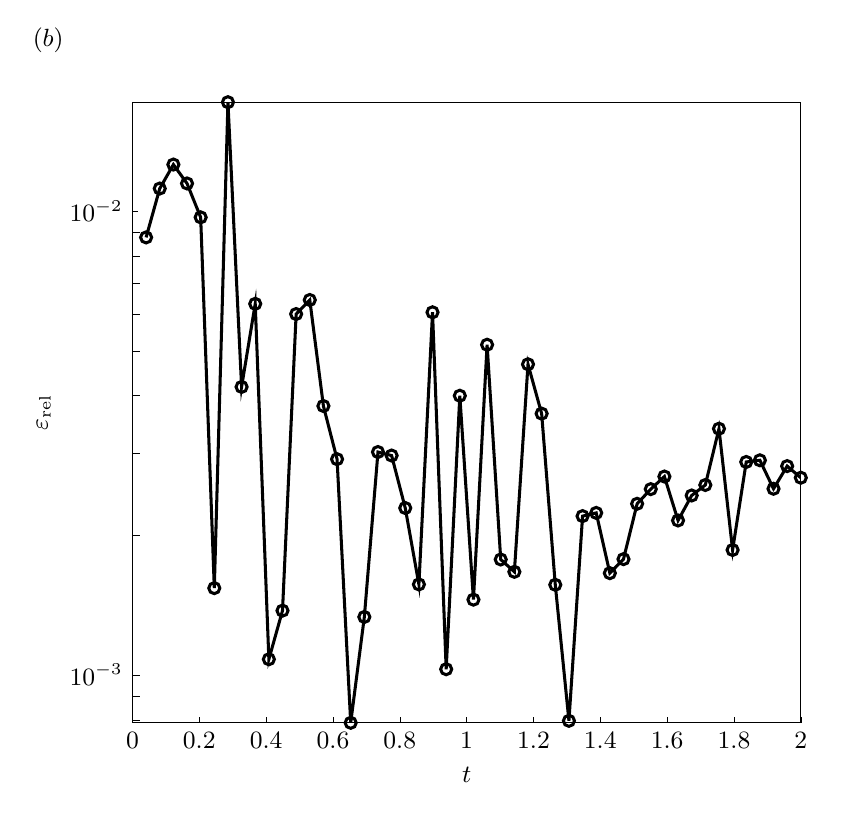
\begin{tikzpicture}

\begin{axis}[%
width=11.252in,
height=7.131in,
at={(1.887in,0.962in)},
scale only axis,
clip=true,
separate axis lines,
every outer x axis line/.append style={black},
every x tick label/.append style={font=\color{black}},
every x tick/.append style={black},
xmin=0,
xmax=2,
xlabel={$t$},
every outer y axis line/.append style={black},
every y tick label/.append style={font=\color{black}},
every y tick/.append style={black},
ymode=log,
ymin=0.000788505972857121,
ymax=0.0171877742818613,
yminorticks=true,
ylabel={$\varepsilon_{\mathrm{rel}}$},
axis background/.style={fill=white},
clip=true,
clip mode=individual,
axis lines=box,
xtick pos=bottom,
ytick pos=left,
tick align=inside,
major tick length=2pt,
width=0.7\linewidth,
height=0.65\linewidth,
every axis/.append style={font=\fontsize{9}{9}\selectfont},xlabel style={font=\fontsize{9}{9}\selectfont},title style={font=\fontsize{9}{9}\selectfont},
legend style={font=\fontsize{8}{9}\selectfont,inner sep=1pt,row sep=1pt,column sep=2pt,nodes={scale=1.00},draw=none},legend image post style={xscale=0.35},
legend columns=1,
scaled x ticks=false,
tick label style={/pgf/number format/fixed,/pgf/number format/precision=2},
every x tick label/.append style={font=\fontsize{9}{9}\selectfont\color{black}},
every y tick label/.append style={font=\fontsize{9}{9}\selectfont\color{black}},
,,
colormap={sigmamap}{rgb(0.0000)=(0.0200,0.1880,0.3800); rgb(0.1000)=(0.0743,0.3456,0.5616); rgb(0.2000)=(0.1918,0.4980,0.7060); rgb(0.3000)=(0.3890,0.6708,0.8226); rgb(0.4000)=(0.7552,0.8682,0.9228); rgb(0.5000)=(0.9690,0.9689,0.9689); rgb(0.6000)=(0.9425,0.8044,0.7614); rgb(0.7000)=(0.8767,0.4910,0.4020); rgb(0.8000)=(0.7869,0.2866,0.2470); rgb(0.9000)=(0.6186,0.1239,0.1568); rgb(1.0000)=(0.4040,0.0000,0.1220)}
]
\addplot [color=black, line width=1.1pt, mark size=2.0pt, mark=o, mark options={solid, black}, forget plot]
  table[row sep=crcr]{%
0.0408163265306122	0.00878209811562205\\
0.0816326530612245	0.0111941806492774\\
0.122448979591837	0.0126101851991099\\
0.163265306122449	0.0114811782204232\\
0.204081632653061	0.00970313334920131\\
0.244897959183673	0.00153902173259956\\
0.285714285714286	0.0171877742818613\\
0.326530612244898	0.00417974437950421\\
0.36734693877551	0.00631468530853708\\
0.408163265306122	0.00108087480641458\\
0.448979591836735	0.00137606782422971\\
0.489795918367347	0.00600284974065746\\
0.530612244897959	0.00643647684440219\\
0.571428571428571	0.00380239451954645\\
0.612244897959184	0.00291963380726255\\
0.653061224489796	0.000788505972857121\\
0.693877551020408	0.00133358609120693\\
0.73469387755102	0.00302530234874586\\
0.775510204081633	0.00297246497902733\\
0.816326530612245	0.00229060726278548\\
0.857142857142857	0.00156751459559027\\
0.897959183673469	0.00605437664190624\\
0.938775510204082	0.00102870291992012\\
0.979591836734694	0.00400052873076924\\
1.02040816326531	0.00145329962832689\\
1.06122448979592	0.00515350795621087\\
1.10204081632653	0.00177419523894462\\
1.14285714285714	0.00166862247912742\\
1.18367346938776	0.00467701383645614\\
1.22448979591837	0.00366070578064619\\
1.26530612244898	0.00156472793820272\\
1.30612244897959	0.0007962865886255\\
1.3469387755102	0.00220022155439051\\
1.38775510204082	0.00223567046606397\\
1.42857142857143	0.00165761528769134\\
1.46938775510204	0.00177711338366069\\
1.51020408163265	0.00233929710023111\\
1.55102040816327	0.00251588724675035\\
1.59183673469388	0.00267844283941867\\
1.63265306122449	0.00215323446866404\\
1.6734693877551	0.00243766286825963\\
1.71428571428571	0.0025679319084316\\
1.75510204081633	0.00339645302008812\\
1.79591836734694	0.00186001446540253\\
1.83673469387755	0.00287954246870691\\
1.87755102040816	0.00290346172621076\\
1.91836734693878	0.00252045629313518\\
1.95918367346939	0.00282068740684575\\
2	0.00266261335982454\\
};
\node[right, align=left, inner sep=0]
at (rel axis cs:-0.15,1.1) {$(b)$};
\end{axis}
\end{tikzpicture}%
    \end{minipage}
    \caption{Non-autonomous verification of the SSTE estimator. \((a)\) Normalized mean energy growth \(g(T)\) compared with the closed-form prediction. \((b)\) Relative error of the SSTE estimate as a function of final time.}
    \label{fig:nonautonomous_hutchpp}
\end{figure}
We finally validate the SSTE construction against a fully non-autonomous linear problem for which \(g(T)\) is available in closed form. The model problem is
\begin{equation}
  b(t)\frac{\partial q}{\partial t}
  =
  a(t)\frac{\partial^2 q}{\partial z^2}
  -
  c(t)\frac{\partial q}{\partial z}
  +
  r(t)q .
\end{equation}
The initial covariance is chosen as
\begin{equation}
  C_{00}^{z}(z,z')
  =
  \exp\left(
    -\frac{(z-z')^2}{\lambda^2}
  \right).
\end{equation}
For this model, the transport term only shifts the solution and does not affect the spatially integrated covariance. The normalized mean energy growth is therefore
\begin{equation}
  g(T)
  =
  \frac{\tr\left\{\mathsfbi{C}(T)\right\}}{\tr\left\{\mathsfbi{C}(0)\right\}}
  =
  \frac{
    \exp\left(2S(T)\right)
  }{
    \sqrt{1+8\tau(T)/\lambda^2}
  },
  \qquad
  \tau(T)=\int_0^T \frac{a(t)}{b(t)}\,dt,
  \qquad
  S(T)=\int_0^T \frac{r(t)}{b(t)}\,dt .
\end{equation}
This provides a direct reference for the matrix-free SSTE estimate. In the numerical test shown below, the interval is \(z\in[-64,64)\), discretized with \(N=256\) periodic grid points. The first and second spatial derivatives are approximated with eighth-order periodic finite-difference matrices, giving \(\mathsfbi{B}(t)=b(t)\mathsfbi{I}\) and \(\mathsfbi{A}(t)=a(t)\mathsfbi{D}_2-c(t)\mathsfbi{D}_1+r(t)\mathsfbi{I}\). The trace is evaluated with the uniform quadrature weight \(\Delta z\), which cancels in the normalized comparison. The final time range is \(0\le T\le 2\), with time-step target \(\Delta t=0.01\), and the initial covariance length is \(\lambda=0.5\). The scalar coefficients are
\begin{equation}
  a(t)=0.2+0.8e^{-t/5},\qquad
  c(t)=0.25+0.15\cos(1.3t),
\end{equation}
\begin{equation}
  r(t)=0.5\sqrt{t}+0.04\sin(0.9t),\qquad
  b(t)=1.0+0.2\sin(0.7t).
\end{equation}
The SSTE estimate uses \(50\) probes.
